\begin{frame}
  \frametitle{关键字}
  \begin{itemize}
    \item 定义:事先定义的,有特别意义的单词,被Java语言保留下来有着特殊含义和用途,所以有时又叫保留字
    \item 所由的Java关键字都是小写
    \item \texttt{goto}和\texttt{const}虽目前未被Java使用,但是依旧是保留关键字
    \item 一般情况下,IDE编辑器会将关键字以特殊高亮的形式展现
  \end{itemize}
  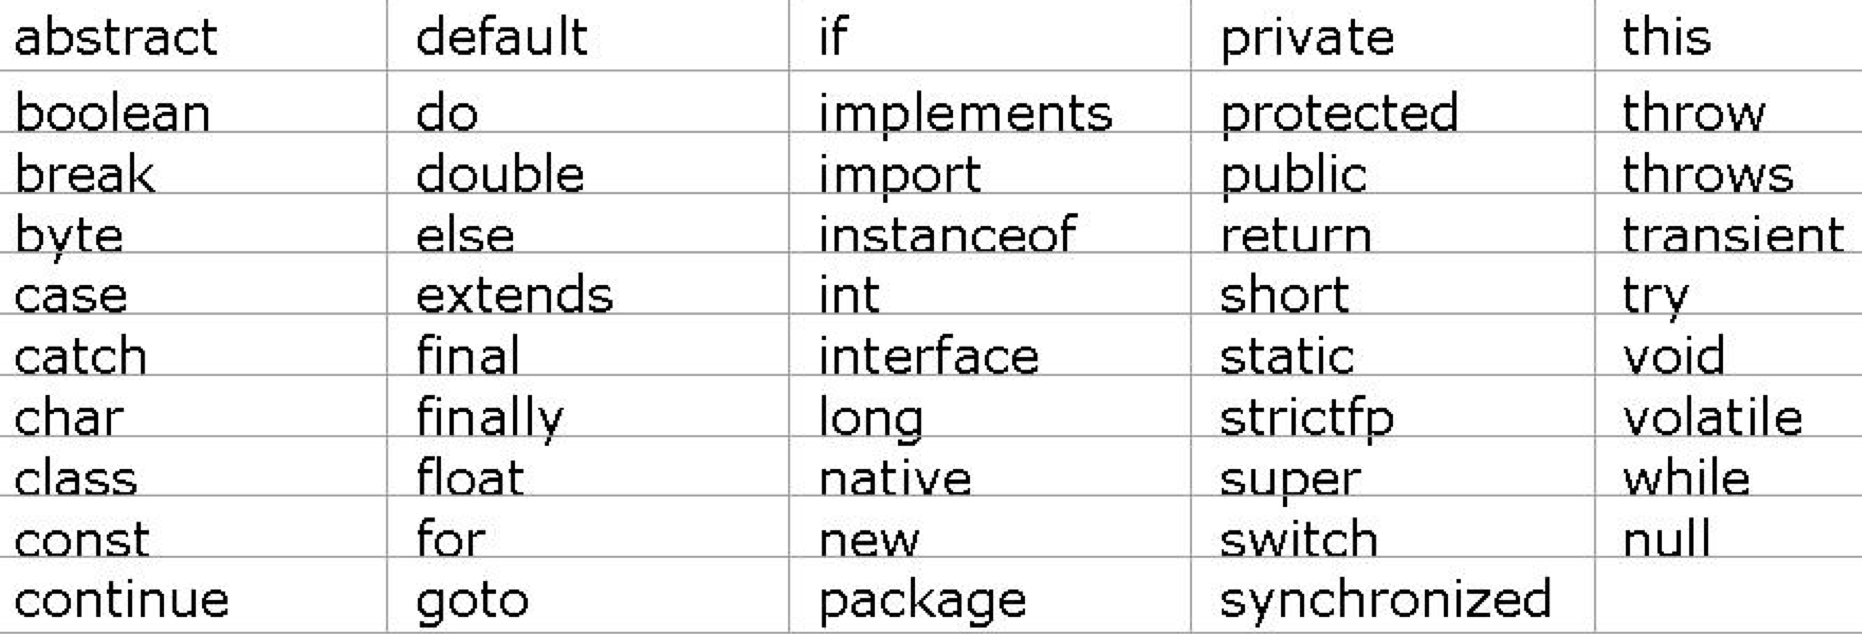
\includegraphics[width=\textwidth]{figures/keywords}
\end{frame}

\begin{frame}
  \frametitle{标识符}
  \begin{itemize}
    \item 定义:用于给Java程序中变量、类、方法等要素命名的字符串序列
    \item Java标识符规则:
      \begin{itemize}
        \item 只能由字母、数字、下划线“\_”、美元符"\$"号组成
        \item 不能以数字开头,只能以字符、下划线、美元符号开头
        \item 不能是Java中的关键字
        \item 大小写敏感
      \end{itemize}
    \item 通俗地说,凡是可以自己起名字的地方,都要遵守标识符规则
    \item 标志符中的字母指Unicode中的字母,不光包括英文26个字母,甚至包括中文的汉字、希腊字母、日文片假名等
    \item 合法标志符举例:\texttt{myName,My\_name,Points,\$points,\_sys\_ta,OK,\_23b,\_3\_}
    \item 非法标志符举例:\texttt{\#name,25name,class,\&time,if}
  \end{itemize}
\end{frame}

\begin{frame}[fragile]
  \frametitle{变量}
  \begin{itemize}
    \item 变量是Java中最基本的数据存储单元,其要素包括:变量名、变量的数据类型和作用域
    \item 变量必须先声明,后使用,声明格式为:\java|type varName [= valValue]|
    \begin{javacode}
      String a; //声明了一个变量,但未赋值,相当于C中的空指针
      int i = 100; //声明了一个变量,并为其赋值
      double a, b, c = 1.1; //一次赋值三个变量
    \end{javacode}
    \item 本质上讲,Java中的变量其实就是内存中的一小块区域,这块区域可以使用变量名来访问
  \end{itemize}
\end{frame}

\begin{frame}
  \frametitle{Java中的数据类型}
  \begin{itemize}
    \item Java中共两大类数据类型:基本数据类型和引用数据类型
    \item 引用数据类型实际就是C语言中的指针引用!Java中除了基本数据类型,其它本质上都是指针!
    \item Java函数的参数如果是基本数据类型,那么传值调用;如果是引用类型,则本质上是传址调用!
  \end{itemize}
  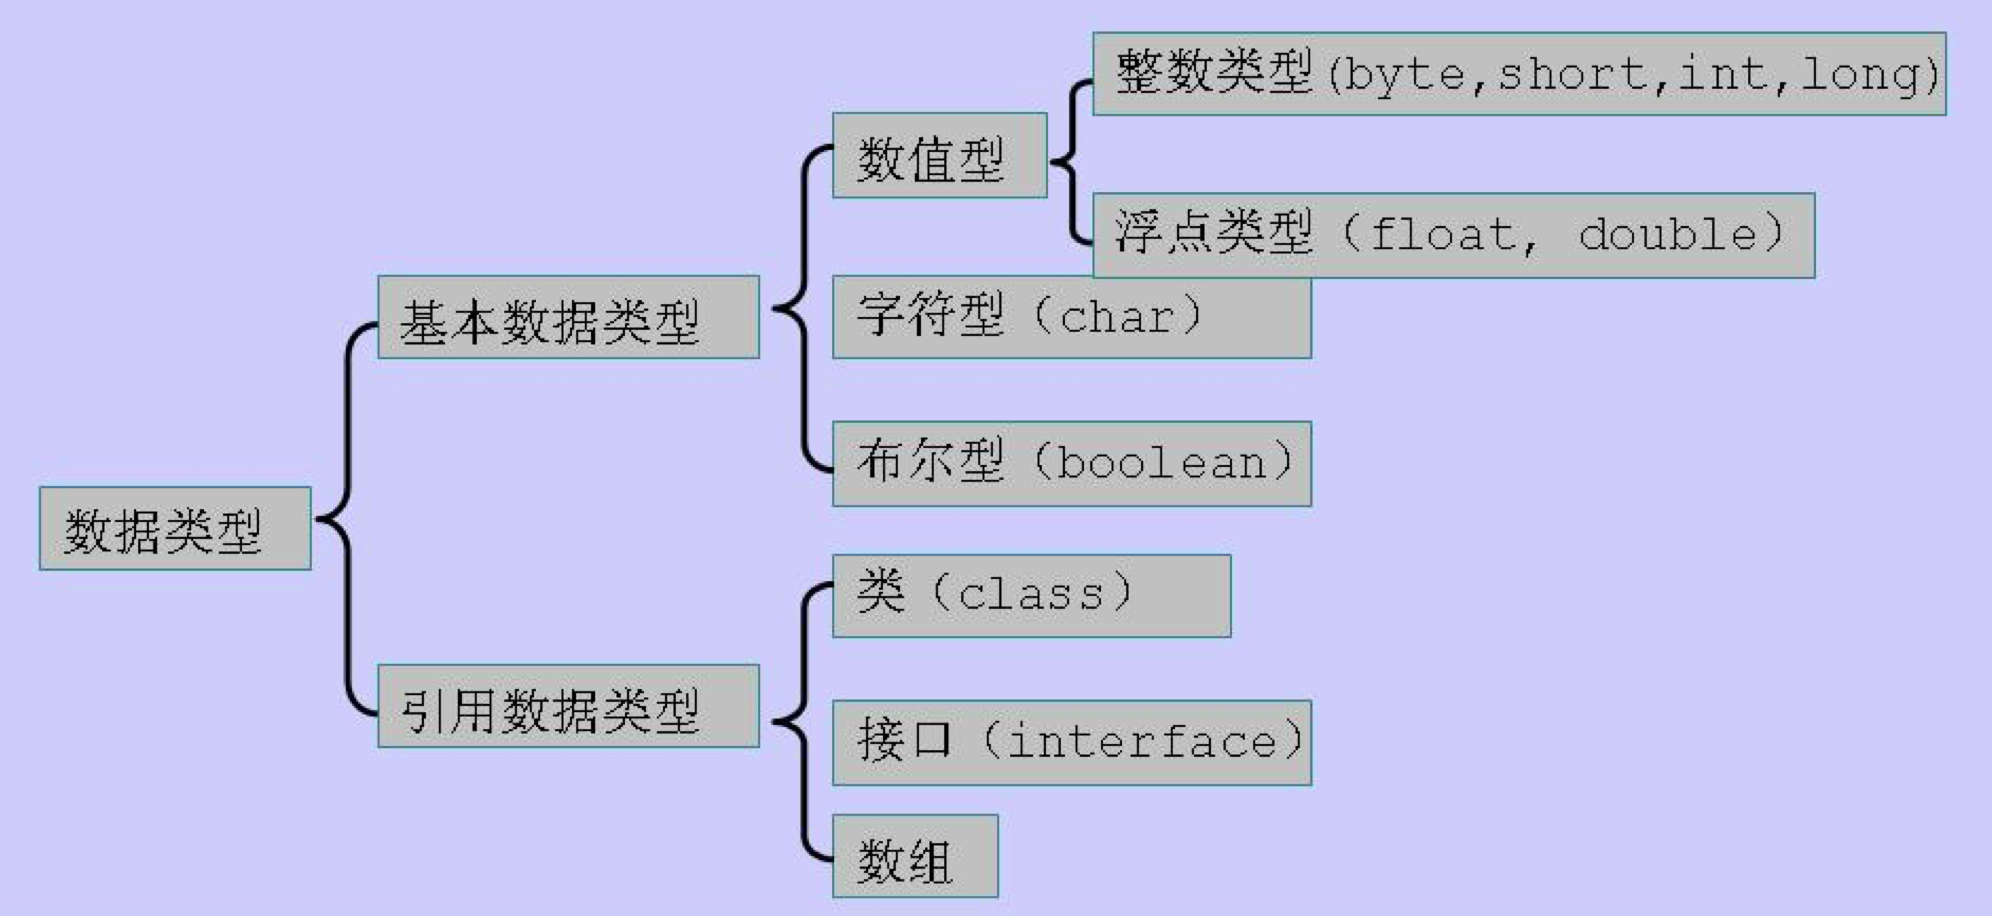
\includegraphics[width=\textwidth]{figures/data_types}
\end{frame}

\begin{frame}
  \frametitle{数字型}
  \begin{itemize}
    \item 
  \end{itemize}
\end{frame}

\begin{frame}
  \frametitle{为什么“1/2=0”?}
  \begin{itemize}
    \item 
  \end{itemize}
\end{frame}

\begin{frame}[fragile]
  \frametitle{布尔型}
  \begin{itemize}
    \item 布尔型数据用于逻辑运算,一般用于程序流程控制,使用\texttt{boolean}声明一个布尔型变量
    \item Java中的布尔型数据只能取两个值\texttt{true}和\texttt{false},不能使用0或者null来表示(注意此处和和C语言不同)
  \end{itemize}
  \begin{javacode}
    boolean a = true;
    boolean b = false;
    
    if (a) { //使用布尔型数据用于流程控制
    }
    
    boolean c = 0; //错误,Java中布尔型只能取true或者false
    
    int d = -1;
    if (d) { //错误,Java中只能使用布尔型做为程序流程控制
    }
  \end{javacode}
\end{frame}

\begin{frame}[fragile]
  \frametitle{字符型}
  \begin{itemize}
    \item 字符型数据表示一个字符,用单引号\texttt{'}包围(注意不能用双引号,双引号包围的是字符串!)
    \item Java字符采用Unicode编码,每个字符占用两个字节(称码点),所以字符类型数据可以转换为整数型数据
    \item Unicode编码的字符不光包含了AsicII字符,还包含了很多外语的字母,如汉字等
    \item 允许使用反斜杠来表示具有特殊意义的字符
  \end{itemize}
  \begin{javacode}
    char a = 'x';
    char b = "x"; //错误,双引号括起来的表示字符串
    char c = 'abc'; // 错误,字符型数据只能是1个字符
    char d = '\n'; //表示一个换行符
    char e = '1';// e是一个字符型数据,不是一个整数!
    char f = '中'; //Java中的字是Unicode编码的字符,包括中文
    char f = '\u0061'; // 采用Unicode的形式给字符赋值
  \end{javacode}
\end{frame}

\begin{frame}
  \frametitle{数字型}
  \begin{itemize}
    \item 
  \end{itemize}
\end{frame}

\begin{frame}
  \frametitle{字符和字符串的区别}
  \begin{itemize}
    \item 字符只能包含一个字母,而字符串是一个或多个字母的有序集合
    \item 字符使用单引号,而字符串使用双引号
    \item \javainline{char}是一个关键字,而字符串\javainline{String}是一个类
    \item 字符可以通过强制类型转换变为与之对应的数字,而字符串不可以
    \item 字符串不等同于字符数组!
  \end{itemize}
\end{frame}

\begin{frame}
  \frametitle{数组}
  \begin{itemize}
    \item 数组是多个\textbf{相同}类型数据的集合
    \item 和C语言中的数组类似,Java中的数组本质上也是一个指针,属于Java的引用类型,做为函数参数是进行传址调用
    \item 声明方式(建议使用第一种方法,更为明了):\java|type[] valName|或\java|type valName[]|
    \item 声明数组时不能指定其元素个数!只有创建时可以指定元素个数!
  \end{itemize}
\end{frame}

\begin{frame}[fragile]
  \frametitle{数组的创建和初始化}
  \begin{javacode}
   //数组的创建
  int[] arr1 = new int[5];
  
  //数组的动态初始化
  for (int i=0;i<5;i++) {
    arr1[i] = i; 
  }
  
  //数组的静态初始化
  int[] arr2 = {1, 2, 3};
  \end{javacode}

\end{frame}

\begin{frame}
  \frametitle{数组的基本操作}
  \begin{itemize}
    \item 获得数组的元素个数:
    \java|arr.length|
    \item 获得数组指定位置的元素:
    \java|arr[i]|
    \item 数组从0开始索引,获得数组的最后一个元素:
    \java|arr[arr.length - 1]|
    \item 如果数组的长度为$L$,则当访问不在$[0, L]$范围内的元素时,会出现\javainline{IndexOutOfBoundsException}错误(数组索引越界错误)
    \item 访问未被赋值的元素时,返回\javainline{null}
  \end{itemize}
\end{frame}

\begin{frame}[fragile]
  \frametitle{关键字null}
  \begin{itemize}
    \item 关键字\javainline{null}表示“空”的概念
    \item 访问\javainline{null}时,会报空针错误\javainline{NullPointerException}
    \item \javainline{null}不等于\javainline{false},请使用\javainline{a == null}判断一个变量是否为空!
  \end{itemize}
  \begin{javacode}
    int[] a = {1, 2, 3};
    //请问下行会报错么?
    int x = a[3]; 
    
    int[] b = new int[3];
    b[0] = 1;
    //请问下行会报错么?
    int y = b[1] + 1;
  \end{javacode}
\end{frame}

\begin{frame}[fragile]
  \frametitle{读取终端用户的输入参数}
  \begin{itemize}
    \item Java将用户输入的参数保存在main方法的args参数中
    \item args参数是一个字符串数组,每个元素是一个用户输入的参数
  \end{itemize}
  \begin{javacode}
    public static void main(String[] args) {

    }
  \end{javacode}

\end{frame}

\begin{frame}[fragile]
  \frametitle{二维数组}
  \begin{itemize}
    \item 可以看出组成元素为数组的数组
    \item 声明和初始化应当遵循从高维到低维的顺序
  \end{itemize}
  \begin{javacode}
    int[][] a = new int[3][];
    int[][] b = {{1,2}, {3, 4}};
    int[][] c = new int[][3]; //非法!
  \end{javacode}
\end{frame}

\begin{frame}
  \frametitle{实验一:累加器}
  读取终端输入的数字并求和
\end{frame}









